% Source: graduate-coursework/Research/Intro_to_Agents/handouts/Part7_Parallelization.tex

\documentclass[border=4pt]{standalone}
\usepackage{amsmath,amssymb,amsfonts}
\usepackage[T1]{fontenc}
\usepackage{graphicx}
\usepackage{lmodern}
\usepackage{tikz}
\usepackage{xcolor}
\usetikzlibrary{shapes.geometric, arrows.meta, positioning, calc, fit, backgrounds, matrix, decorations.pathreplacing}

\definecolor{UofSCGarnet}{HTML}{73000a}
\definecolor{UofSCBlack}{HTML}{000000}
\definecolor{UofSCWhite}{HTML}{ffffff}
\definecolor{UofSCRose}{HTML}{CC2E40}
\definecolor{UofSCAtlantic}{HTML}{466A9F}
\definecolor{UofSCCongaree}{HTML}{1F414D}
\definecolor{UofSCHorseshoe}{HTML}{65780B}
\definecolor{UofSCGrass}{HTML}{CED318}
\definecolor{UofSCHoneycomb}{HTML}{A49137}
\definecolor{UofSC90Black}{HTML}{363636}
\definecolor{UofSC70Black}{HTML}{5C5C5C}
\definecolor{UofSC50Black}{HTML}{A2A2A2}
\definecolor{UofSCWarmGrey}{HTML}{676156}
\definecolor{UofSCSandstorm}{HTML}{FFF2E3}
\definecolor{UofSCDarkGarnet}{HTML}{570008}
\definecolor{UofSCAzalea}{HTML}{844247}

\tikzset{
    % Node styles - all with sharp corners
    agentbox/.style={
        rectangle,
        draw=UofSCGarnet,
        fill=UofSCSandstorm,
        thick,
        minimum width=2cm,
        minimum height=0.8cm,
        text centered,
        font=\footnotesize
    },
    processbox/.style={
        rectangle,
        draw=UofSCAtlantic,
        fill=UofSCWhite,
        thick,
        minimum width=2.5cm,
        minimum height=0.7cm,
        text centered,
        font=\footnotesize
    },
    syncbox/.style={
        rectangle,
        draw=UofSCCongaree,
        fill=UofSCCongaree!20,
        thick,
        minimum width=3cm,
        minimum height=0.5cm,
        text centered,
        font=\footnotesize\bfseries
    },
    resultbox/.style={
        rectangle,
        draw=UofSCHorseshoe,
        fill=UofSCGrass!30,
        thick,
        minimum width=2cm,
        minimum height=0.7cm,
        text centered,
        font=\footnotesize
    },
    % Arrow styles
    myarrow/.style={
        ->,
        >=Stealth,
        thick,
        UofSCBlack
    },
    dashedarrow/.style={
        ->,
        >=Stealth,
        thick,
        dashed,
        UofSC70Black
    },
    % Timeline styles
    timeline/.style={
        draw=UofSCBlack,
        thick,
        ->,
        >=Stealth
    },
    timeblock/.style={
        rectangle,
        draw=none,
        minimum height=0.5cm,
        text centered,
        font=\tiny
    }
}

\begin{document}
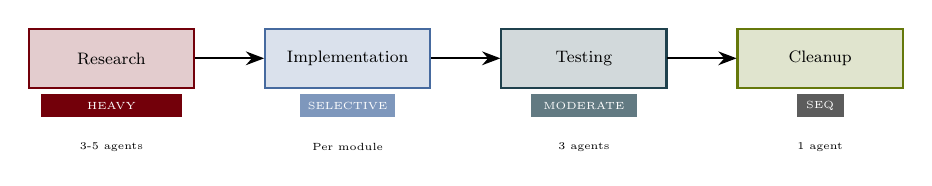
\begin{tikzpicture}[scale=0.75, transform shape]
            % Phase boxes
            \node[rectangle,draw=UofSCGarnet,thick,fill=UofSCGarnet!20,minimum width=2.8cm,minimum height=1cm] (research) at (0,0) {\footnotesize Research};
            \node[rectangle,draw=UofSCAtlantic,thick,fill=UofSCAtlantic!20,minimum width=2.8cm,minimum height=1cm] (impl) at (4,0) {\footnotesize Implementation};
            \node[rectangle,draw=UofSCCongaree,thick,fill=UofSCCongaree!20,minimum width=2.8cm,minimum height=1cm] (test) at (8,0) {\footnotesize Testing};
            \node[rectangle,draw=UofSCHorseshoe,thick,fill=UofSCHorseshoe!20,minimum width=2.8cm,minimum height=1cm] (clean) at (12,0) {\footnotesize Cleanup};

            % Parallelization intensity bars
            \fill[UofSCGarnet] (0-1.2,-1) rectangle (0+1.2,-0.6);
            \node[font=\tiny,white] at (0,-0.8) {HEAVY};

            \fill[UofSCAtlantic!70] (4-0.8,-1) rectangle (4+0.8,-0.6);
            \node[font=\tiny,white] at (4,-0.8) {SELECTIVE};

            \fill[UofSCCongaree!70] (8-0.9,-1) rectangle (8+0.9,-0.6);
            \node[font=\tiny,white] at (8,-0.8) {MODERATE};

            \fill[UofSC70Black] (12-0.4,-1) rectangle (12+0.4,-0.6);
            \node[font=\tiny,white] at (12,-0.8) {SEQ};

            % Arrows
            \draw[myarrow] (research.east) -- (impl.west);
            \draw[myarrow] (impl.east) -- (test.west);
            \draw[myarrow] (test.east) -- (clean.west);

            % Agent indicators
            \node[font=\tiny] at (0,-1.5) {3-5 agents};
            \node[font=\tiny] at (4,-1.5) {Per module};
            \node[font=\tiny] at (8,-1.5) {3 agents};
            \node[font=\tiny] at (12,-1.5) {1 agent};
        \end{tikzpicture}
\end{document}
